\documentclass[a4paper,12pt]{article}
\usepackage{geometry}
\geometry{margin=1in}
\usepackage{enumitem}
\usepackage{graphicx}

\begin{document}

\title{Exercice sur le Système de Fichiers}
\author{Votre Nom}
\date{\today}
\maketitle

\section*{I. Le Système de Fichiers}

\subsection*{I.1 Utiliser le Système de Fichiers}

\begin{enumerate}[label=\textbf{Question \arabic*:}]
    \item Question_1 :Ouvrez un terminal en tant qu’utilisateur : sudo su  :
    \begin{enumerate}
        \item afichage du nom de connexion \\ 
        \textbf{Réponse :} {whoami} \\
        \item a/Votre UID (IDentifiant Utilisateur) et GID (IDentifiant de Groupe). \\ 
        \textbf{Réponse :} {id} \\
        \item b/Votre UID (IDentifiant Utilisateur) et GID (IDentifiant de Groupe). \\ 
        \textbf{Réponse :} {hostname} \\
        \item c/Le nom de la machine de connexion. \\ 
        \textbf{Réponse :} {hostname} \\
        \item d/La liste des utilisateurs connectés à la même machine que vous. \\ 
        \textbf{Réponse :} {hostname} \\
        \item Le nom du répertoire courant. \\ 
        \textbf{Réponse :} {hostname} \\
        \item La liste de tous les fichiers du répertoire courant (fichiers cachés compris). \\ 
        \textbf{Réponse :} {hostname} \\
    \end{enumerate}
        \textbf{Image :} 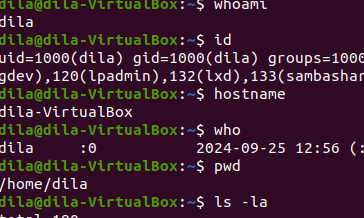
\includegraphics[width=0.3\textwidth]{totale.png} % Remplacez par le nom de votre image
        
        

        \item Positionnez-vous sous le sous-répertoire de nom local du répertoire /usr. \\ 
        \textbf{Réponse :} {hostname} \\
        \textbf{Image :} 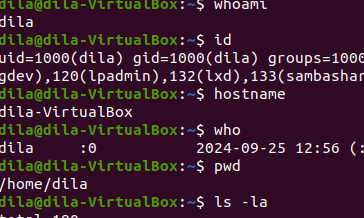
\includegraphics[width=0.3\textwidth]{totale.png} % Remplacez par le nom de votre image
        
        \item Positionnez-vous sous votre répertoire de connexion. \\ 
        \textbf{Réponse :} {} \\
        \textbf{Image :} 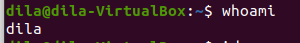
\includegraphics[width=0.3\textwidth]{who.png} % Remplacez par le nom de votre image
    \end{enumerate}
\end{enumerate}

\end{document}

\documentclass[a4paper,12pt]{article}
\usepackage{geometry}
\geometry{margin=1in}
\usepackage{enumitem}
\usepackage{graphicx}

\begin{document}

\title{Exercice sur le Système de Fichiers}
\author{Votre Nom}
\date{\today}
\maketitle

\section*{I. Le Système de Fichiers}

\subsection*{I.1 Utiliser le Système de Fichiers}

\begin{enumerate}[label=\textbf{Question \arabic*:}]
    \item Ouvrez un terminal en tant qu’utilisateur  ==> sudo su :
    \begin{enumerate}
        \item Votre nom de connexion. \\ 
        \textbf{Réponse :} \texttt{whoami} \\
        \item a/Votre UID (IDentifiant Utilisateur) et GID (IDentifiant de Groupe). \\ 
        \textbf{Réponse :} \texttt{id} \\

        \item c/Le nom de la machine de connexion. \\ 
        \textbf{Réponse :} \texttt{hostname} \\

        \item d/La liste des utilisateurs connectés à la même machine que vous. \\ 
        \textbf{Réponse :} \texttt{who} \\

        \item Le nom du répertoire courant. \\ 
        \textbf{Réponse :} \texttt{pwd} \\

        \item La liste de tous les fichiers du répertoire courant (fichiers cachés compris). \\ 
        \textbf{Réponse :} \texttt{ls -a} \\ 
    \end{enumerate}

    \item Positionnez-vous sous le sous-répertoire de nom local du répertoire /usr. \\ 
\textbf{Réponse :} \texttt{cd /usr/local} \\ 

\item Positionnez-vous sous votre répertoire de connexion. \\ 
\textbf{Réponse :} \texttt{cd ~} \\ 

\item Affichez la liste de tous les fichiers de chacun des répertoires /usr/local/bin, /bin et /usr/share, en utilisant la désignation absolue ou relative. \\ 
\textbf{Réponse :} 
\begin{itemize}
    \item \texttt{ls /usr/local/bin}
    \item \texttt{ls /bin}
    \item \texttt{ls /usr/share}
\end{itemize} \\ 

\end{enumerate}

\end{document}






1.	MASSIANI Louis-Paul 